\documentclass[twocolumn,10pt]{article}

\usepackage[english]{babel}
\usepackage[utf8]{inputenc}
\usepackage[T1]{fontenc}
\usepackage{listings}
\usepackage{graphicx}
\usepackage{comment}
\usepackage{hyperref}


\title{Assessed Coursework 1 Report\linebreak Advanced Programming 3 }

\author{Willian de Oliveira Barreiros Junior}

\begin{document}
\maketitle

\section{Introduction}

This coursework is divided into three major parts: the implementation of \textbf{date.c}, the implementation of \textbf{tldlist.c} using the binary search tree as the list structure, and finally, upgrading the binary tree structure in \textbf{tldlist.c} to an AVL tree. 

The source code from this coursework can also be found at
\url{https://github.com/WillianJunior/AdvancedProgramming3Project1},.

\section{Date}

The date structure consists of only one 32 bit integer that contains the day, month and year of the given date, shown by Listing \ref{lst:date_struct}.

\begin{lstlisting}[language=C, caption={Date struct}, label=lst:date_struct]
typedef struct date Date;

struct date {
	int32_t date_bit;
};
\end{lstlisting}

Given that the day, month and year fields have to be between 1 and 31, 1 and 12 , and 0 and 9999, respectively, we can represent the fields as a 5 bits integer, a 4 bit integer and a 14 bit integer. The order of the fields is shown by Figure \ref{fig:date_bit}.

\begin{figure}[h]
\centering
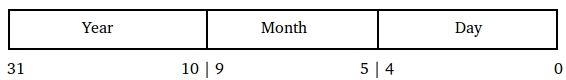
\includegraphics[scale=0.35]{img1.jpg}
\caption{Bitmap of the date integer}
\label{fig:date_bit}
\end{figure}

Using that order the comparison between two dates is the same as a two integers comparison. The assemble of \textbf{date\_{}bit}, given the year, month and day is also fairly easy, using only addition and shifting operations as we can see in Listing \ref{lst:date_bit}.

\begin{lstlisting}[language=C, caption={Assemble of date\_{}bit}, label=lst:date_bit]
	date_bit = year;
	
	date_bit <<= 4;
	date_bit += month;

	date_bit <<= 5;
	date_bit += day;
\end{lstlisting}

\section{Binary Search Tree}

The next step done was the implementation of a list of TLDs using a binary search tree (BST). The structure used can be seen in Listing \ref{lst:tld_bin_str}. 

In order to make the hostname count easier and more efficient \textbf{tldlist} has a counter of sucesfull insertions called \textbf{host\_{}count}, which is incremented after each insertion.

Also, there aren't repeated hostnames in the BST. A hostname counter is used in each node of the BST. This way is also very efficient when inserting a valid hostname and returning the number of hostnames added.

\begin{lstlisting}[language=C, caption={Structs of the TLD binary tree}, label=lst:tld_bin_str]
typedef struct tldlist TLDList;
typedef struct tldnode TLDNode;
typedef struct tlditerator TLDIterator;

struct tldlist {
	TLDNode *root;
	long host_count;
	Date *begin;
	Date *end;
};

struct tldnode {
	char *hostname;
	long host_count;
	TLDNode *left;
	TLDNode *right;
	TLDNode *parent;
};

struct tlditerator {
	TLDNode *node;
};
\end{lstlisting}

The BST was defined as a double linked tree structure. This was done to make the iteration more straightforward. The iteration strategy is defined by Listing \ref{lst:iter}.

Another factor to be taken into consideration when chosing the iteration strategy is the destruction of the list. The iterator was implemented to travel throught the left subtree, the right subtree and finaly the given node, in this order. This way the destruction of the list is as simple as iterate throught the tree freeing the nodes.

Since we are working with an ordered structure, it is also interesting to have an ordered iterator. Given that the first iterator implementation is needed for the destruction of the tree a second iterator was implemented.

 
\begin{lstlisting}[caption={Iteration strategy}, label=lst:iter]
Iterator constructor:
1. Find the leftmost node (lesser  value)
2. Return new iterator pointing to  the aforementioned node

Iteration:
1. If the current node is NULL return  null
2. If the current node is the root of  the BST, set the return node as the  current node, set the current node to  null and return the return node.
3. Set the curent node as the return  node
4. If the curent node is the left node  and the parent have a right node, than  the new current node is the leftmost  node begining from the parent's right  node
5. Otherwise, the new current node is  the current node's parent
6. Return the return node

\end{lstlisting}

Since the list structure is a BST, the insertion operation is trivial. In order to insert a hostname we first perform a search for that hostname. Since we are working with a tree, the search is performed recursively. If there already is the hostname the \textbf{host\_{}count} is incremented, otherwise a new node is created.

\section{AVL Upgrade}

Given that we have a working BST, the effort to upgrade it to an AVL BST isn't much. The upgrade was divided into the folowing steps: update the structs, implement the basic AVL functions (right and left rotation, and height calculator), implement the height updater and node balancing functions given the basic functions, and finally, linking the AVL functions to the BST implementation.

\subsection{Struct}

The only diference between the BST and the AVL structs is that a height field is needed into the \textbf{tldnode} struct.

\subsection{Basic Functions}

The most basic function is the height calculation, which returns zero if the pointer is NULL, or returns the greater value of the children nodes plus one.

The other functions needed are the rotations. Since the node struct have a reference to its parent, there is no need for auxiliary variables. The most troublesome part of the rotations involves the root node. When the rotation modifies the root node the \textbf{TLDList} variable has to change its root reference too. There are two ways to perform this update: passing the reference of the \textbf{TLDList} variable throught the AVL functions in order to the update happen as soon as the root node is changed, or to return the root node from every AVL function and only when it reached the top level (the BST new node function) the current root would be compared to the returned root. Since not on every insertion there is a rotation, the strategy chosen was to pass the reference of the \textbf{TLDList} variable.

\subsection{AVL Balance Tree Function}

After the insertion of a node on the tree the first step is to update the height of the tree. This is done easily given that we have the parent node reference. The update is done by calling the above-mentioned height calculator on a given node and then setting the current node to its parent, until it reach the root.

Finaly, given that the tree was balanced before the last insertion we need to check if the tree is still balanced and perform rotations when needed. The simplification of the balance algorithm for a given node is shown in the Listing \ref{lst:balance_tree}

\begin{lstlisting}[language=C, caption={Balance Algorithm}, label=lst:balance_tree]
if node_height < 2
   return // no balancing required

balance factor = node->left->height  - node->right->height

if |balance_factor| < 2
   return // no balancing required

if balance_factor > 0
  if node->left->right->height > 
     node->left->left->height
       // left-right case
       rotate_left(node->left)
       rotate_right(node)
  else
     // right-right case
     rotate_right(node)
else
  if node->right->left->height >
     node->right->right->height
       // right-left case
       rotate_right(node->right)
       rotate_left(node)
  else
     rotate_left(node)
\end{lstlisting}

In order to balance the whole tree we need to apply the algorithm shown in the Listing \ref{lst:balance_tree} in all parent nodes, setting the current node as its parent after each check, until we hit the root.

\subsection{Linking the AVL functions to the BST}

Now that we have the two high level AVL functions we can finally upgrade the BST to an AVL tree. This can be easily done by calling the update height and balance tree functions in this order on the new node.

\section{Tests}

To make sure that the program produced in this assignment was correct, four tests were performed: Basic unit test, Debugging test, and testing using the text files given on the assignment handout. 

The unit test were performed to check the functionality of the date module only.

After the implementation of the AVL BST module the algorithm was set to be verbose (i.e. to print as much information about the tree structure as possible). This was performed to validate that the tree was in fact balanced.

Finally, the program was tested using the two given text files, the smallest with 12 entries and the largest with 10095 entries. All the tests were successful.

\end{document}
